\documentclass[11pt,a4paper,twoside,french,svgnames]{report}
\usepackage[utf8]{inputenc} % force the use of utf8
\usepackage[T1]{fontenc} % font encoding, allows accents
\usepackage[papersize={21cm,29.7cm},top= 2.5cm,bottom=2.5cm, inner=2.5cm, outer=2.5cm]{geometry} % page formatting
\usepackage[francais]{babel} % translate everything in the desired language: table of contents, etc. 'english' can be replaced with 'francais'
\usepackage{graphicx} % images management
\usepackage{wrapfig} % floating images
\usepackage{array} % allow arrays
\usepackage{fancyhdr} % headers/footers management (overrides empty, plain and headings)
\usepackage{listings} % code insertion (MUST BE WRITTEN AFTER BABEL)
%\usepackage[nottoc,numbib]{tocbibind} % bib in toc
%\usepackage{pdfpages} % include PDF documents
\usepackage{enumitem} % for /setlist
\usepackage{color,soul} % add some colors and hightlight
\usepackage{xcolor} % more colors
\usepackage[hyphens]{url} % auto break lines in URL
\usepackage[hidelinks,  colorlinks  = true, % no borders, colors enabled
                        anchorcolor = blue,
                        linkcolor   = black, % links in table of contents
                        urlcolor    = blue,
                        citecolor   = blue]{hyperref}
%\usepackage[%nonumberlist,% no page number
%            toc,% displayed in toc
%            numberedsection,% displayed as a numbered section in toc
%            xindy]{glossaries} % glossary with xindy style. MUST BE WRITTEN AFTER HYPERREF
%\setglossarystyle{listgroup}

\sethlcolor{cyan} % package soul
\newcommand{\file}[1]{\hl{\emph{#1}}} % highlight a file URI

%\makeglossaries
%\loadglsentries{glossary.tex}

%%%%%%%%%%%%%%%%%%%%%%%%%%%%%%%%%%%%%%%%%%%%%%%%%%%%%%%% LISTINGS %%%%%%%%%%%%%%%%%%%%%%%%%%%%%%%%%%%%%%%%%%%%%%%%%%%%%%%%
\definecolor{comment}{rgb}{0.12, 0.38, 0.18 } % adjusted, in Eclipse: {0.25, 0.42, 0.30 } = #3F6A4D
\definecolor{keyword}{rgb}{0.37, 0.08, 0.25}  % #5F1441
\definecolor{string}{rgb}{0.06, 0.10, 0.98} % #101AF9

\lstset{
  columns=flexible, %prevent extra spaces
  rulecolor=\color{black!50},
  backgroundcolor = \color{blue!10},
  numbers=none, % line numbering
  showspaces=false,
  showtabs=false,
  tabsize=4,
  breaklines=true,
  showstringspaces=false,
  breakatwhitespace=false,
  commentstyle=\color{comment},
  keywordstyle=\color{keyword},
  stringstyle=\color{string},
  basicstyle=\ttfamily,
  extendedchars=true,
  emph=[2]{In},
  emphstyle=[2]\color{black!70},
  morecomment=[l][\color{blue}]{Out},
  frame=single,
  frameround=tttt,
  framerule=0.3pt,
  framesep=4pt,
  belowcaptionskip=2.1pt,
  literate={à}{{\`a }}1 {â}{{\^a}}1 %                         letter a
           {À}{{\`A}}1 {Â}{{\^A}}1 %                         letter A
           {ç}{{\c{c}}}1 %                                   letter c
           {Ç}{{\c{C}}}1 %                                   letter C
           {é}{{\'e}}1 {è}{{\`e}}1 {ê}{{\^e}}1 {ë}{{\"e}}1 % letter e
           {É}{{\'E}}1 {È}{{\`E}}1 {Ê}{{\^E}}1 {Ë}{{\"E}}1 % letter E
           {î}{{\^i}}1 {ï}{{\"i}}1 %                         letter i
           {Î}{{\^I}}1 {Ï}{{\"I}}1 %                         letter I
           {ô}{{\^o}}1 %                                     letter o
           {Ô}{{\^O}}1 %                                     letter O
           {œ}{{\oe}}1 %                                     letter oe
           {Œ}{{\OE}}1 %                                     letter OE
           {ù}{{\`u}}1 {û}{{\^u}}1 {ü}{{\"u}}1 %             letter u
           {Ù}{{\`U}}1 {Û}{{\^U}}1 {Ü}{{\"U}}1 %             letter U
  % above is a hack to force UTF8 compatibility (only for french)
}

\newcommand{\textcode}[1]{\lstset{
  title={{\setlength{\fboxsep}{1pt}\fcolorbox{orange}{yellow!20}{\sffamily\scriptsize
              \textcolor{gray!10}{\_}{#1}\textcolor{gray!10}{\_}}}}
  }
}

\newcommand{\clanguage}{\lstset{
  language=C,
  title={{\setlength{\fboxsep}{1pt}\fcolorbox{orange}{yellow!20}{\sffamily\scriptsize
              \textcolor{gray!10}{\_}C\textcolor{gray!10}{\_}}}}
  }
}
%%%%%%%%%%%%%%%%%%%%%%%%%%%%%%%%%%%%%%%%%%%%%%%%%%%%%%%%%%%%%%%%%%%%%%%%%%%%%%%%%%%%%%%%%%%%%%%%%%%%%%%%%%%%%%%%%%%%%%%%%%%

%\parindent=20pt
\fancypagestyle{plain}{
    % Headers
    \fancyhead[R]{Rapport UTComputer}
    \fancyhead[L]{Jérôme \textsc{COSTE} - Gabriel \textsc{HURTADO}}

    % Footers
    \renewcommand{\footrulewidth}{0.1pt}
    \fancyfoot[C]{Université de Technologie de Compiègne}
    \fancyfoot[LE]{\ifnum\thepage>0 \thepage \fi}
    \fancyfoot[RO]{\ifnum\thepage>0 \thepage \fi}
}

\fancypagestyle{empty}{%
    \renewcommand{\headrulewidth}{0pt} % No sub line
    \fancyhead{} % Empty the header

    \renewcommand{\footrulewidth}{0pt}
    \fancyfoot{}
} 

\setlist[itemize,2]{label={$\bullet$}} % use bullets for nested itemize

% First page
\newcommand{\presentation}[1]{\vspace{0.3cm}\large{\textbf{#1}}\vspace{0.3cm}\\}
\newcommand{\presentationLarge}[1]{\vspace{0.3cm}\LARGE{\textbf{#1}}\vspace{0.3cm}\\}

% Overrides chapter (numbered and no-numbered) headings: remove space, display only the title
\makeatletter
  \def\@makechapterhead#1{%
  \vspace*{0\p@}% avant 50
  {\parindent \z@ \raggedright \normalfont
    %\ifnum \c@secnumdepth >\m@ne
    %    \huge\bfseries \@chapapp\space \thechapter
    %    \par\nobreak
    %    \vskip 20\p@
    %\fi
    \interlinepenalty\@M
    \Huge \bfseries \thechapter\quad #1   
    \vskip 40\p@
  }}
  \def\@makeschapterhead#1{%
  \vspace*{0\p@}% before 50
  {\parindent \z@ \raggedright
    \normalfont
    \interlinepenalty\@M
    \Huge \bfseries  #1\par\nobreak
    \vskip 40\p@
  }}
\makeatother

\newcommand{\ignore}[1]{} % inline comments

\pagenumbering{arabic}
%\addtocounter{page}{-7} % page numbering starts at 1 + (-7)
\pagestyle{plain} % uses fancy

\title{Rapport LO21}
\author{Anaïs NEVEUX et Romain PELLERIN}
\date\today

%\setcounter{tocdepth}{4}

\begin{document}
\thispagestyle{empty} % only for the current page

\begin{center}

\includegraphics[height=3cm]{UTC_logo.png}\\
\vspace{2.5cm}
\presentation{Université de Technologie de Compiègne} 
\presentation{LO21}

\vspace{2cm}
\noindent\fbox{
\begin{minipage}{0.9\textwidth}
\begin{center}
    \presentationLarge{Rapport de projet}
    \presentationLarge{\Huge{UTComputer}}
\end{center}
\end{minipage}}
\vspace{3cm}

\presentation{Printemps 2016}
\vspace{1cm}

\def\arraystretch{1.5} % 1 is the default
\begin{tabular}{|>{\hfill\arraybackslash}p{5cm}|p{5cm}|}
\hline
    \multicolumn{2}{|c|}{Jérome \textsc{COSTE} - Gabriel \textsc{HURTADO}}\\
\hline
    \multicolumn{2}{|c|}{\textit{\today}}\\% dates
\hline
\end{tabular}
\end{center}

\tableofcontents

\part{Projet et architecture}

\chapter{Objectifs}

L'objectif de ce projet était de réaliser une calculatrice utilisant la notation RPN.

\bigskip

Dans le cadre du projet de LO21, nous avons été chargé de la programmation de ce logiciel et de son interface.
\medskip

Cette calculatrice devait être capable de gérer tout types de nombres, mais aussi des programmes simples, et des variables. Elle devait par ailleurs comporter une interface graphique, avec une vue principale comportant la pile, le champ de saisie de commande ainsi que divers  boutons, mais aussi des vues secondaires.


\section{Équipe et organisation}

Le projet était constituée de deux étudiants :

\begin{itemize}
  \item Jérôme \textsc{Coste}, étudiant en GI02
  \item Gabriel \textsc{Hurtado}, étudiant en GI02
\end{itemize}

\medskip
Etant relativement peu expérimentés dans le domaine de la programmation orientée objet, nous nous sommes beaucoup servis des notions aquises lors de l'UV LO21, notamment au niveau des design patterns.

\bigskip

Au niveau des outils, nous avons utilisé :

\begin{itemize}
    \item \textbf{Draw.io} : l'outil en ligne, permettant la mise en ligne d'une version collaborative de notre UML
   \item \textbf{Qt Creator} : l'IDE, environnement de développement, permettant la création facilité d'applications fenêtrées
   \item \textbf{Qt Designer}: cet environnement de création d'interface graphique à simplifier la mise en forme de celle-ci
\end{itemize}

\section{Répartition du travail}

Au vu de la charge importante de travail, il à été nécessaire de trouver une organisation satisfaisante. Lors d'une étape préliminaire, nous avons travaillés en collaboration sur la modélisation du problème, en étudiant ensemble les différents design patterns et les différentes solutions qui en découlaient. Suite à cette phase de modélisation, nous avons mis en place un repository sur Github, et nous nous somme répartis les différents "blocs" de notre UML. Jérôme s'est principalement occupé de l'interprétation des commandes saisies, de l'interface graphique, de la gestion des littérales, de la pile et des opérateurs Undo et Redo. Gabriel, s'est occupé des différents opérateurs, de la sauvegarde et restauration du contexte lors de l'échec d'opérations, ainsi que de la gestion des variables. Certaines parties ont été faites en collaboration, comme les expressions, et les littérales.



\section{Réunions hebdomadaires}

Pour mener à bien efficacement ce projet, nous avons choisi d'utiliser une méthode Agile: SCRUM

\medskip

SCRUM repose sur des sprints, qui sont des périodes de travail généralement étalée sur une à plusieurs semaines avec des objectifs précis clairement définis au début de chaque période. Nous avons travaillé d'un façon très similaire, avec des réunions au moins hebdomadaires.

\section{Git}

Notre \textit{workflow} était principalement basé sur l'outil Git, couplé à la plateforme web Github. Cela offrait plusieurs avantages indéniables :

\begin{itemize}
      \item Reporter les bugs facilement en ouvrant des tickets. La fonctionnalité s'appelle \textit{Issues} sur Github. Ainsi, dès que quelqu'un repérait un bug, dû à du code écrit par cette même personne ou quelqu'un d'autre, nous ouvrions un ticket. Cela permettait de suivre l'évolution de la résolution de bugs et d'en garder une trace.
      \item Le travail à distance était grandement facilité: il est possible de travailler conjointement sur un même document, grâce aux outils de résolution des conflits.
   
\end{itemize}




\chapter{Choix d'architecture}

La premier travail à effectuer, étant donné que le cahier des charges exprime clairement les besoins, a été un travail de modélisation de notre architecture. L'utilisation d'une pile pour le stockage, couplée au design pattern Mémento pour la gestion des sauvegardes de la pile, nous a semblé évident.
\newline \newline
La hiérarchisation des classes dérivant de la classe \textit{littérale} était clairement exprimée dans le sujet. Nous avons ainsi choisi de modéliser une classe \textit{littérale complexes}, qui exclue les programmes, atomes et expressions. Ces \textit{littérales complexes} ont pour particularité d'exprimer des nombres. Ainsi ces littérales partagent certaines similitudes telles que la possibilité d'une méthode renvoyant leur négation. \newline 
Les \textit{littérales numériques} caractérisent toutes les \textit{littérales complexes} n'étant pas des complexes. Même si à ce niveau  de hiérarchisation, cette classe n'apporte aucun avantage technique, elle permet de décrire très simplement un complexe comme composé de deux \textit{littérales numériques}. Il en est de même pour la classe \textit{littérale simple} qui n'offre pas non plus d'avantage technique, mais permet de bien exprimer la structure.
\newline 
Comme un dessin vaut 1000 mots, voici la hiérarchisation complète des littérales

\begin{figure}[h]
    \centering
    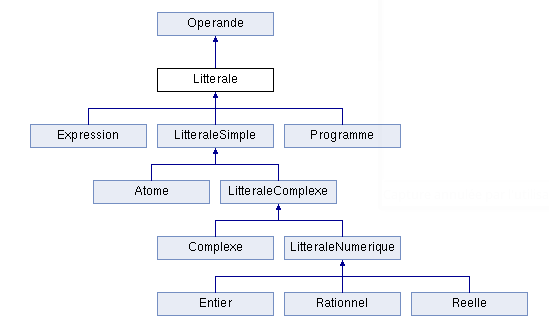
\includegraphics[height = 7cm]{hierarchie_litterale.png}
    \caption{Hiérarchisation des littérales}
    \label{fig:my_label}
\end{figure}

L'un des points de la conception, qui s'est révélé être le plus délicat a été la modélisation des opérateurs. Nous avions tout d'abord opté pour la surcharge d'opérateurs, car il s'agit d'un outil formidable de la programmation Orientée Objet, mais en étudiant le nombre de combinaisons possibles à traiter, et en réfléchissant à la souplesse de cette solution, nous nous sommes rendu compte qu'elle n'était pas viable. Nous avons alors opté pour des opérateurs sous forme d'objets instanciables, qui sont beaucoup plus faciles à maintenir.
La hiérarchie des classes d'opérateur se base sur un héritage multiple. Une partie de l'héritage exprime l'arité de l'opérateur (unaire ou binaire), et l'autre partie exprime son type (conditionnel, numérique, pile,...). L'avantage d'une telle conception est que chaque classe mère apporte ce qui est nécessaire.
Par exemple, la classe OpérateurBinaire apporte deux attributs littérale* . 
\newline \newline
La modélisation d'un contrôleur qui coordonne la pile les opérateurs et les littérales, ainsi que la modélisation de l'interface graphique et des variables, ont émergées durant la phase de programmation, car il nous fallait avant tout définir clairement comment seraient construit les littérales et les opérateurs à partir d'une chaine de caractère
\newline \newline
Nous avons donc opté pour deux "factory", une pour les opérateurs et une pour les littérales, qui prenaient en entrée une chaîne de caractère, afin de produire le bon opérateur ou la bonne littérale en sortie.
\newline \newline
La phase de conception s'est achevée sur cette réflexion.

L'UML présent en annexe témoigne de l'état de la conception avant le début de la programmation.

\chapter{Fonctionnement de la calculatrice}
Dans cette partie nous allons voir plus en détail le fonctionnement de routine principale de la calculatrice en supposant l'arrivée d'une opération sur la ligne de commande

\section{Le contrôleur}
La méthode getNextCommande() de l'interface principale s'occupe d'envoyer la chaîne de caractère tapée dans la ligne de commande graphique au contrôleur via sa méthode commande().
\newline \newline
Ce dernier doit alors trouver le premier mot de la chaîne envoyée, grâce à la méthode firstWord() du contrôleur (fonctionnement détaillé dans la documentation). Suite à cela, il tente de fabriquer une littérale à partir du premier mot via la LitteraleFactory. Si celle-ci renvoie nullptr, la fabrication à échouée , sinon la littérale obtenue est empilée. Dans tous les cas le contrôleur tente ensuite de fabriquer un opérateur avec ce même mot en l'envoyant dans l'OpérateurFactory. Si celle-ci renvoie nullptr, la fabrication a aussi échouée, sinon il demande à l'opérateur d'effectuer son opération. Ensuite, le contrôleur passe au mot suivant jusqu'à qu'il finisse.

\section{La LitteraleFactory}
La LitteraleFactory est appelée par le contrôleur via la méthode creerRPNLitterale. Il reçois une String, et demande à la méthode getRPNExample() de lui fournir un exemple de littérale construit sur ce modèle. La méthode gerRPNExample() cherche alors parmi tout les symboles enregistrés, par ordre de priorité, un qui existe dans la string donnée. Dès qu'il trouve, il renvoie l'exemple de littérale associé au symbole. La méthode creerRPNLitterale se charge alors d'appeler la méthode getFromString() de la littérale avec la string, pour recevoir une copie de la littérale, chargée avec les valeurs de la string.

\section{L'OpérateurFactory}
Celle ci cherche juste à faire correspondre la string avec un symbole d'opérateur connu. S'il trouve, il prends l'exemple associé à cette littérale et en demande une copie, qu'il renvoie au contrôleur.


\section{Ce qu'il manque}
Par manque de temps nous avons préféré privilégier au maximum la gestion de la mémoire, au détriment des opérateurs optionnels. D'autre part, nous avions un doute sur le but de l'opérateur edit, permettant de modifier un programme référencé par un atome sur la pile. Étant donné qu'un atome ne peut être sur la pile que si il n'est pas lié à une variable ou un programme, nous avons choisi de lui faire ouvrir le menu d'édition des programmes.
\medskip
D'autre fonctionnalités n'ont pu être implémentées, faute de temps. Par exemple, quand un opérateur comme + * ou - est saisi sur la "ligne de commande", il n'est pas directement interprété, il est nécessaire de faire "Entrée". Finalement, nous n'avons pas eu le temps d'afficher les délimitateurs gauche et droits de la littérale expression ou programme dans le cas ou elle "déborde"

\part{Adaptabilité}
Au niveau de l'adaptabilité, il était nécessaire de faire un choix. Nous avons considéré que l'ajout de nouveaux opérateurs était bien plus fréquent que l'ajout de nouvelles littérales. Nous avons donc mis l'accent sur la flexibilité des opérateurs, parfois au détriment de celle des littérales.

\section{Adaptabilité des littérales}
La création de littérale peut se faire en héritant au minimum de la classe littérale. Pour enregistrer une nouvelle littérale, il faudra donc définir son comportement pour quelques méthodes comme getFromString(), getCopy(),etc et enregistrer la littérale auprès de la litteraleFactory avec la méthode enregistrer() (ou enregistrerInfix(), si l'on veut qu'elle ne soit comprise que dans des expressions.). L'enregistrement requiert au minimum un symbole et une priorité différente de celles définies de base (visibles dans le fichier main.cpp), mais l'on peut aussi définir la façon dont la littérale est détectée dans le contrôleur, en définissant une classe héritant de WordIdentifier, qui redéfinit les méthodes wordGuesser() qui vérifie que le mot est bon et wordPosition() qui permet l'extraction du mot. On peut bien entendu omettre ce paramètre et le comportement par défaut fait que le mot se fini au prochain espace (ou fin de la ligne de commande).
Ainsi, ces littérales nouvellement ajoutées seront comprises partout. Le seul problème est la compatibilité de celles-ci avec les opérateurs. Leur comportement n'étant pas défini, il faudra modifier directement les opérateurs en question.

\section{Adaptabilité des opérateurs}

L'adaptabilité est l'avantage principal de notre choix d'architecture, au niveau des opérateurs. En effet, si l'utilisateur souhaite définir un nouvel opérateur, il n'a qu'a le faire hériter des classes qui le constitue, et son comportement sera en très grande partie hérité de ces classes supérieures. Par exemple, pour implémenter un opérateur comme sinus, il suffit de le faire hériter d'opérateur numérique, et d'opérateur préfixe. La seule méthode à définir sera \textit{traitementOperateur()}, définissant ce que l'opérateur doit faire de ses deux littérales. Il faudra par la suite enregistrer cet opérateur auprès de sa factory.
Grâce à cette architecture, l'opérateur n'a à s'occuper ni de savoir si elles viennent de la pile, ni à les sauvegarder pour la gestion du contexte. Son seul travail sera de définir le comportement, et éventuellement d'émettre une exception si les littérales reçues sont d'un mauvais type, ou si l'opération demandée est sémantiquement incorrecte.

\medskip
Cependant ce choix d'architecture présente un désavantage. Lors de l'ajout d'une nouvelle littérale, il est nécessaire de modifier une partie des méthodes \textit{traitementOperateur()} des opérateurs pouvant s'appliquer à ce nouveau type de littérale. 
Le désavantage de ce choix d'architecture est clair, mais nous avons considéré qu'il sera très rarement utile de rajouter de nouvelles littérales, et donc qu'il était justifié de privilégier l'adaptabilité des opérateurs.








\part{Annexes}
\begin{figure}[h]
    \centering
    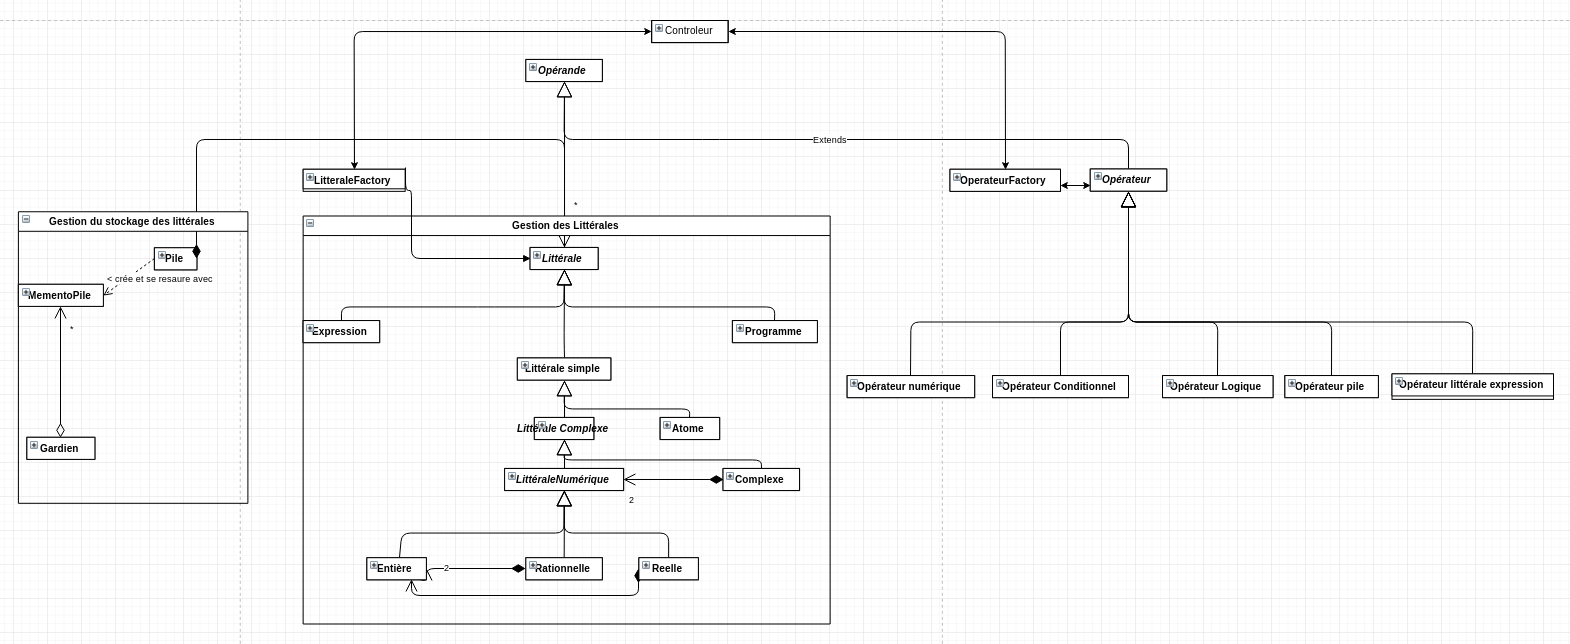
\includegraphics[height = 10cm, angle = 90]{uml.png}
    \caption{Uml initial de notre calculatrice}
    \label{fig:my_label}
\end{figure}

\end{document}